% DistSens_DynResponse.tex

\tikzstyle{Ellipseobject}=[ultra thick, draw=blue, ellipse, minimum width=30em,
    minimum height=8em,align=center]
\tikzstyle{LabelObject}=[draw=black, fill=white,rectangle,rounded corners,line width=0.5mm,%
	  align=center]
\tikzstyle{ArrowObject}=[red,line width=1.0mm, -latex]
\tikzstyle{WingRoot}=[draw=black, fill=white,rectangle,line width=0.25mm,%
	  align=center,minimum width=0.25em,minimum height=4.5em,pattern=north west lines]
\tikzstyle{WingPlanform}=[draw=black, fill=white,rectangle,line width=0.25mm,%
	  align=center,minimum width=14.24em,minimum height=3em]
\tikzstyle{SecObject}=[draw=black, rectangle,line width=0.25mm,%
	  align=center,minimum width=1em,minimum height=3em]
\tikzstyle{SelSecObject}=[draw=black, fill=blue,rectangle,line width=0.25mm,%
	  align=center,minimum width=1em,minimum height=3em]
\tikzstyle{SGObject}=[draw=black, rectangle,line width=0.25mm,%
	  align=center,minimum width=1em,minimum height=1em]
\tikzstyle{SelSGObject}=[draw=black, fill=blue,rectangle,line width=0.25mm,%
	  align=center,minimum width=1em,minimum height=1em]

\resizebox{!}{0.3\textwidth}{
	\begin{tikzpicture}
	  \node[anchor=south west,inner sep=0] (image) at (0,0)%
				{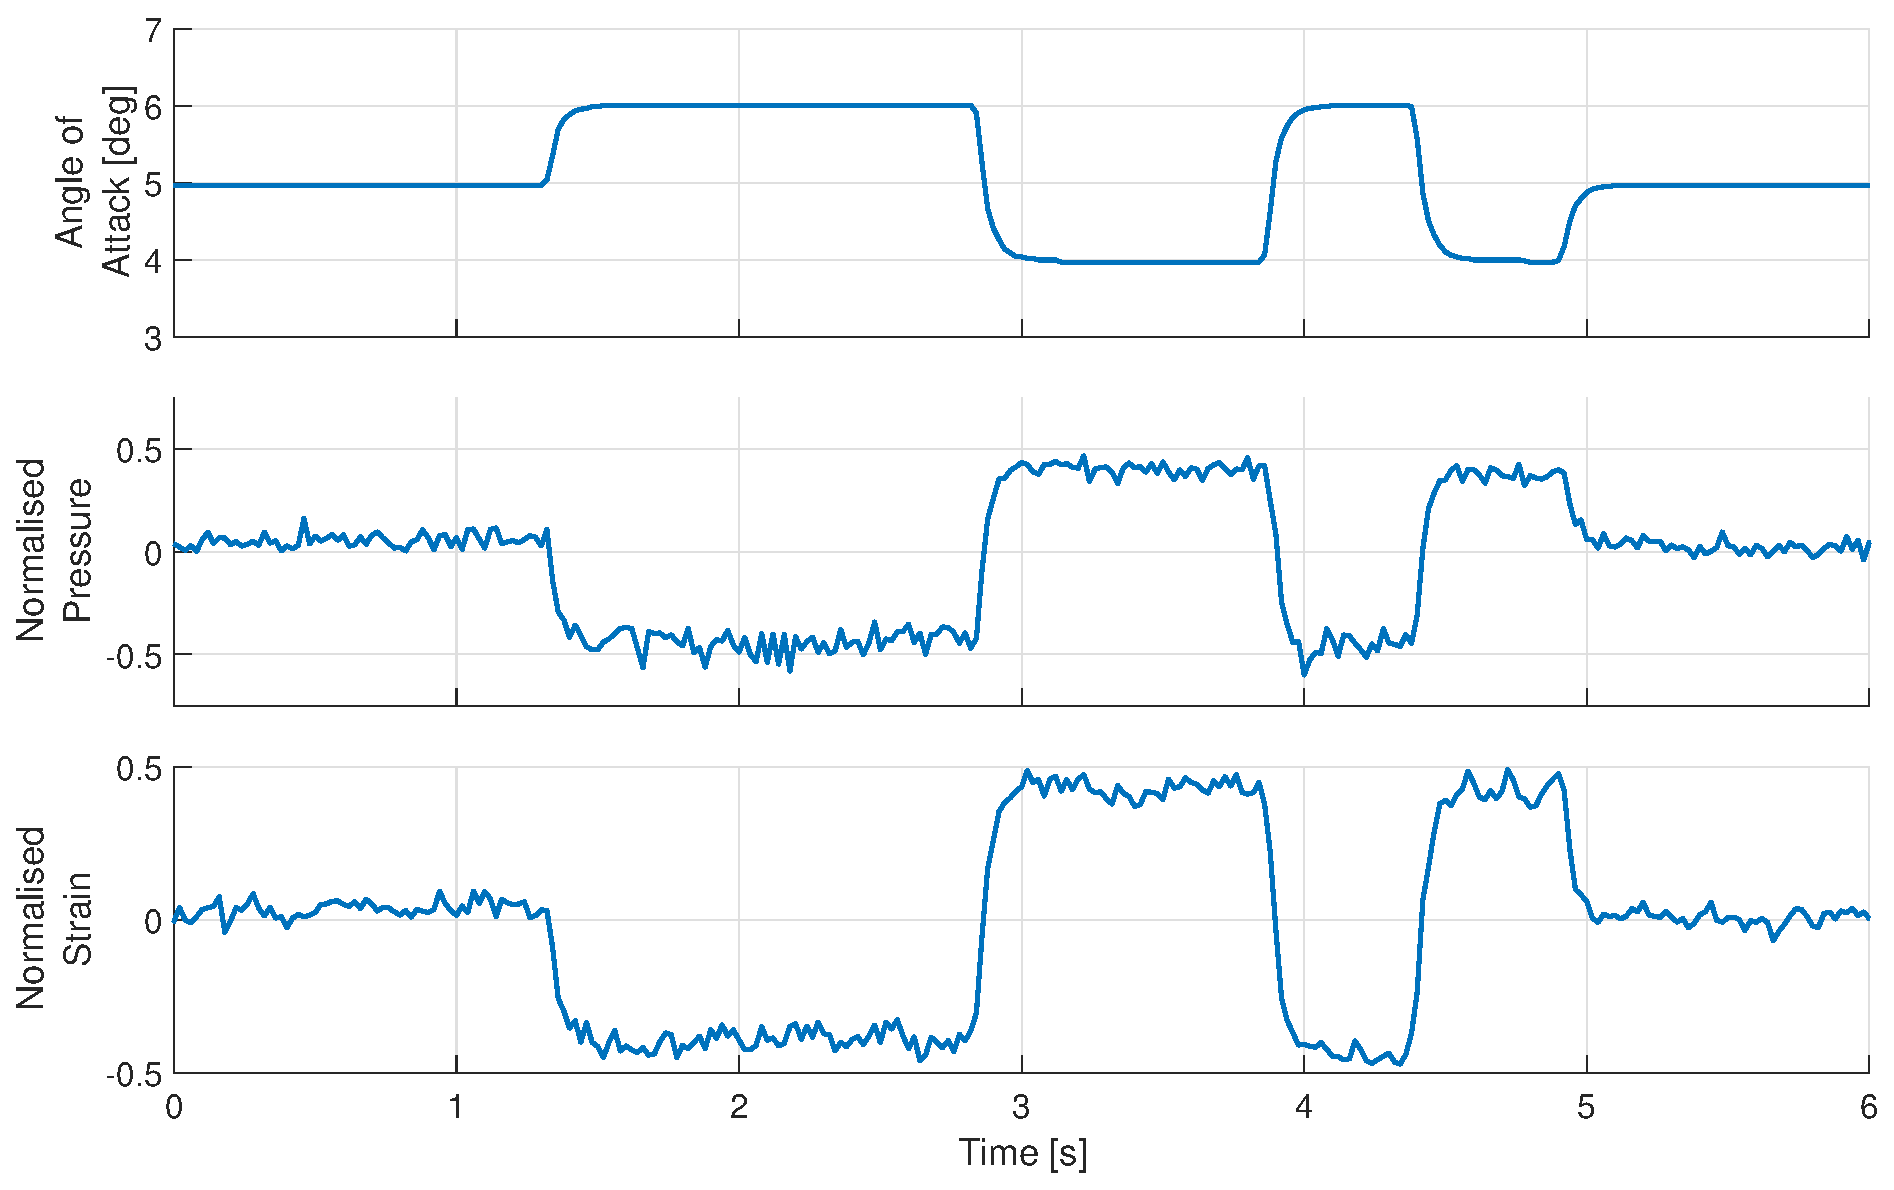
\includegraphics[width=\textwidth]{DistDataSet_P13.eps}};
		% Define scope with 'image' dimensions as reference
		\begin{scope}[x={(image.south east)},y={(image.north west)}]
			%\draw[help lines,xstep=.05,ystep=.05] (0,0) grid (1,1);
			%\foreach \x in {0,1,...,9} { \node [anchor=north] at (\x/10,0) {0.\x}; }
			%\foreach \y in {0,1,...,9} { \node [anchor=east] at (0,\y/10) {0.\y}; }
			
			\only<2>{
			  % Input node
			  \draw(0.575,0.85) node (ServoInput) {};
			  % Input marker
			  \node[Ellipseobject] (ServoInputTimeHist) at (ServoInput) {};
			  % Input label
			  \draw(0.4,0.4) node[LabelObject] (ServoInput_Label) {Rig Servo\\3-2-1-1 Input};
			  % Input arrows
			  \draw[ArrowObject] (ServoInput_Label.north east) -- (ServoInputTimeHist.south);
			}
			\only<3>{
			  % Input node
			  \draw(0.575,0.525) node (PressureResponse) {};
			  % Input marker
			  \node[Ellipseobject] (PressureResponseTimeHist) at (PressureResponse) {};
			  % Input label
			  \draw(0.4,0.15) node[LabelObject] (PressureResponse_Label) {Pressure Response\\Section A ${0.4 c}$ Sensor};
			  % Input arrows
			  \draw[ArrowObject] (PressureResponse_Label.north east) -- (PressureResponseTimeHist.south);
				
				% Airfoil node
			  \draw(0.1,0.85) node (AirfoilNode) {};
				% Airfoil
				\node (Airfoil) at (AirfoilNode) {%
				  \begin{axis}[
					  unit vector ratio*=1 1 1, % keeps a 1:1 scale between x and y axis
					  width=8cm,
						height=3cm,
						xmin=-0.1,
            xmax= 1.1,
						xticklabels={,,},
						yticklabels={,,},
            tick style={draw=none},
						axis on top,
						axis background/.style={fill=white},
						]
				      \addplot[smooth] table [x=x, y=y, col sep=comma] {./Figures/WOT4Airfoil.dat};
							\addplot[smooth,mark=*,blue] plot coordinates {
                (0.4,0.09)
                };
					\end{axis}
				};
				
				% Wing node
			  \draw(0.8,0.905) node (WingNode) {};
			  % Wing instance
			  \node[WingPlanform] (WingPlanform) at (WingNode) {};
				\draw (WingNode) ++(-0.165,0) node[WingRoot] (WingRoot) {};
				\draw (WingNode) ++(-0.075,0) node[SelSecObject] (SecB) {};
				\draw (WingNode) ++(+0.075,0) node[SecObject] (SecA) {};
				\draw (WingNode) ++(-0.115,0) node[SGObject] (SG_A) {};
				\draw (WingNode) ++(-0.045,0) node[SGObject] (SG_B) {};
				\draw (WingNode) ++(+0.045,0) node[SGObject] (SG_C) {};
				\draw (WingNode) ++(+0.115,0) node[SGObject] (SG_D) {};
			}
			\only<4>{
			  % Input node
			  \draw(0.575,0.225) node (StrainResponse) {};
			  % Input marker
			  \node[Ellipseobject] (StrainResponseTimeHist) at (StrainResponse) {};
			  % Input label
			  \draw(0.4,0.6) node[LabelObject] (StrainResponse_Label) {Strain Response\\Section B Inboard Sensor};
			  % Input arrows
			  \draw[ArrowObject] (StrainResponse_Label.south east) -- (StrainResponseTimeHist.north);
				
				% Wing node
			  \draw(0.8,0.905) node (WingNode) {};
			  % Wing instance
			  \node[WingPlanform] (WingPlanform) at (WingNode) {};
				\draw (WingNode) ++(-0.165,0) node[WingRoot] (WingRoot) {};
				\draw (WingNode) ++(-0.075,0) node[SecObject] (SecB) {};
				\draw (WingNode) ++(+0.075,0) node[SecObject] (SecA) {};
				\draw (WingNode) ++(-0.115,0) node[SelSGObject] (SG_A) {};
				\draw (WingNode) ++(-0.045,0) node[SGObject] (SG_B) {};
				\draw (WingNode) ++(+0.045,0) node[SGObject] (SG_C) {};
				\draw (WingNode) ++(+0.115,0) node[SGObject] (SG_D) {};
			}
			
		\end{scope}
	\end{tikzpicture}
}